\documentclass[11pt,a4paper]{article}
\usepackage[margin=2cm]{geometry}
\usepackage[breakable]{tcolorbox}
\usepackage{amsmath,amssymb}
\usepackage{tikz}
\usetikzlibrary{shapes.geometric,arrows.meta,positioning}
\usepackage{enumitem}
\usepackage{graphicx}
\usepackage{hyperref}
\usepackage{array}
\usepackage{booktabs}

% Define custom tcolorbox environments with breakable option
\newtcolorbox{question}[1][]{
    colback=blue!5!white,
    colframe=blue!75!black,
    fonttitle=\bfseries,
    title=Question,
    breakable,
    #1
}

\newtcolorbox{answer}[1][]{
    colback=green!5!white,
    colframe=green!50!black,
    fonttitle=\bfseries,
    title=Answer,
    breakable,
    #1
}

\title{\textbf{Week 4: Statistics \& Probability\\Answers}}
\author{}
\date{}

\begin{document}
\sloppy

\maketitle
\tableofcontents
\newpage

\section{The Monty Hall Problem}

\begin{question}
You are on a game show with 3 doors. Behind one door is a car; behind the other two are goats. You pick a door, say Door 1. The host, Monty Hall, who knows what's behind each door, opens another door (say Door 3) to reveal a goat. He then asks: ``Do you want to switch to Door 2?''

Should you switch?
\end{question}

\begin{answer}
\textbf{YES — you should switch!}

\vspace{0.3cm}
\textbf{Probability Analysis:}
\begin{itemize}
    \item $P(\text{win if you stay}) = \frac{1}{3}$
    \item $P(\text{win if you switch}) = \frac{2}{3}$
\end{itemize}

\vspace{0.3cm}
\textbf{Case Analysis:}

Let's analyse all possible scenarios where you initially pick Door 1:

\begin{center}
\begin{tabular}{|c|c|c|c|c|}
\hline
\textbf{Case} & \textbf{Car Behind} & \textbf{You Pick} & \textbf{Monty Opens} & \textbf{Switch Result} \\
\hline
1 & Door 1 & Door 1 & Door 2 or 3 & \textbf{Lose} (goat) \\
\hline
2 & Door 2 & Door 1 & Door 3 & \textbf{Win} (car) \\
\hline
3 & Door 3 & Door 1 & Door 2 & \textbf{Win} (car) \\
\hline
\end{tabular}
\end{center}

\vspace{0.3cm}
In 2 out of 3 cases, switching wins. Each case has equal probability $\frac{1}{3}$.

\vspace{0.3cm}
\textbf{Why is this counterintuitive?}

The key insight is that \textbf{Monty's action is not random}. He always:
\begin{enumerate}
    \item Opens a door you didn't pick
    \item Opens a door with a goat behind it
    \item Never reveals the car
\end{enumerate}

When you initially pick a door, you have a $\frac{1}{3}$ chance of being correct. The other two doors collectively have a $\frac{2}{3}$ chance of hiding the car. When Monty reveals a goat behind one of those doors, he's effectively concentrating that $\frac{2}{3}$ probability onto the remaining unopened door.

\vspace{0.3cm}
\textbf{Think of it this way:} If you had 100 doors instead of 3, you pick one door ($\frac{1}{100}$ chance), then Monty opens 98 doors showing goats. Would you switch to the one remaining door? Of course! That door now carries $\frac{99}{100}$ probability.
\end{answer}

\newpage
\section{More Examples — Fill in the Blanks}

\subsection*{(a) Will it rain tomorrow?}

\begin{question}
Fill in the table for the experiment: ``Will it rain tomorrow?''
\end{question}

\begin{answer}
\begin{center}
\begin{tabular}{|l|p{10cm}|}
\hline
\textbf{Experiment} & Observe tomorrow's weather \\
\hline
\textbf{Outcome} & Either ``Rain'' or ``No rain'' \\
\hline
\textbf{Sample Space} & $S = \{\text{Rain}, \text{No rain}\}$ \\
\hline
\textbf{Event} & $A = \{\text{Rain}\}$ (the event that it rains) \\
\hline
\end{tabular}
\end{center}

Note: This is a simplified model. In reality, we might have more nuanced outcomes like ``light drizzle'', ``heavy rain'', ``snow'', etc.
\end{answer}

\subsection*{(b) The Birthday Paradox}

\begin{question}
In a room of $n$ people, what is the probability that at least two people share the same birthday?

Complete the analysis for $n = 23$ and $n = 50$.
\end{question}

\begin{answer}
\textbf{Assumptions:} 365 days per year (ignore leap years), birthdays equally distributed.

\vspace{0.3cm}
\textbf{Strategy:} Calculate the probability that \textit{everyone} has different birthdays, then subtract from 1.

\vspace{0.3cm}
Let $P(\text{all different})$ be the probability that all $n$ people have different birthdays:

\begin{align}
P(\text{all different}) &= \frac{365}{365} \times \frac{364}{365} \times \frac{363}{365} \times \cdots \times \frac{365-n+1}{365}\\
&= \frac{365!}{(365-n)! \times 365^n}
\end{align}

Therefore:
\[
P(\text{at least one match}) = 1 - P(\text{all different})
\]

\vspace{0.3cm}
\textbf{Calculations:}

\begin{center}
\begin{tabular}{|c|c|c|}
\hline
\textbf{People ($n$)} & \textbf{$P$(at least one match)} & \textbf{Percentage} \\
\hline
23 & 0.507 & \textbf{50.7\%} \\
\hline
50 & 0.970 & \textbf{97.0\%} \\
\hline
\end{tabular}
\end{center}

\vspace{0.3cm}
\textbf{Surprising result:} With just 23 people, there's already a greater than 50\% chance of a birthday match! With 50 people, it's almost certain (97\%).

\vspace{0.3cm}
\textbf{Why is this counterintuitive?}

People often think: ``There are 365 days and only 23 people, so matches should be rare.'' But we're not asking if someone matches \textit{your} birthday — we're asking if \textit{any pair} matches. With 23 people, there are $\binom{23}{2} = 253$ possible pairs to compare!
\end{answer}

\newpage
\section{Roulette Board (European, 37 pockets)}

European roulette has 37 pockets: numbers 0 through 36. The 0 is green. Of the numbers 1--36: half (18) are red, half (18) are black; half (18) are even, half (18) are odd. Note: 0 is considered neither even nor odd for betting purposes.

\subsection*{(a) Sample Space}

\begin{question}
How many pockets are there? Write the sample space $S$.
\end{question}

\begin{answer}
There are \textbf{37 pockets}.

\[
S = \{0, 1, 2, 3, \ldots, 36\}
\]

Each outcome (where the ball lands) is equally likely with probability $\frac{1}{37}$.
\end{answer}

\subsection*{(b) Colour and Parity Breakdown}

\begin{question}
How many pockets are red? Black? Green? Even? Odd?
\end{question}

\begin{answer}
\begin{center}
\begin{tabular}{|l|c|}
\hline
\textbf{Category} & \textbf{Count} \\
\hline
Red & 18 \\
\hline
Black & 18 \\
\hline
Green & 1 (only 0) \\
\hline
Even & 18 (not including 0) \\
\hline
Odd & 18 \\
\hline
\end{tabular}
\end{center}

Note: The number 0 is green and is \textit{not} counted as even or odd in roulette betting rules.
\end{answer}

\subsection*{(c) Probability of Red}

\begin{question}
What is $P(\text{red})$?
\end{question}

\begin{answer}
\[
P(\text{red}) = \frac{\text{number of red pockets}}{\text{total pockets}} = \frac{18}{37}
\]
\end{answer}

\subsection*{(d) Probability of Even}

\begin{question}
What is $P(\text{even})$?
\end{question}

\begin{answer}
\[
P(\text{even}) = \frac{18}{37}
\]
\end{answer}

\subsection*{(e) Probability of Red OR Even}

\begin{question}
What is $P(\text{red OR even})$?
\end{question}

\begin{answer}
Use the \textbf{union rule}:
\[
P(A \cup B) = P(A) + P(B) - P(A \cap B)
\]

Let $A = \text{red}$ and $B = \text{even}$.

First, identify $P(\text{red AND even})$: the red even numbers are 2, 4, 6, 8, 10, 12, 14, 16, 18, 20, 22, 24, 26, 28, 30, 32, 34, 36 — that's \textbf{8 numbers} (actually, let me recount: the even reds are indeed 8).

Actually, among 1--36, there are 18 evens and 18 odds. Half of the 18 reds are even, so 9 are even — wait, let me recalculate properly.

Red numbers in European roulette: 1, 3, 5, 7, 9, 12, 14, 16, 18, 19, 21, 23, 25, 27, 30, 32, 34, 36.

Even reds: 12, 14, 16, 18, 30, 32, 34, 36 — that's \textbf{8 numbers}.

So:
\begin{align}
P(\text{red OR even}) &= P(\text{red}) + P(\text{even}) - P(\text{red AND even})\\
&= \frac{18}{37} + \frac{18}{37} - \frac{8}{37}\\
&= \frac{28}{37}
\end{align}
\end{answer}

\subsection*{(f) Probability of Red OR Black}

\begin{question}
What is $P(\text{red OR black})$?
\end{question}

\begin{answer}
Red and black are \textbf{mutually exclusive} (a pocket cannot be both red and black).

\[
P(\text{red OR black}) = P(\text{red}) + P(\text{black}) = \frac{18}{37} + \frac{18}{37} = \frac{36}{37}
\]

This is the probability of \textit{not} landing on 0 (green).
\end{answer}

\subsection*{(g) Probability of Red AND Even}

\begin{question}
What is $P(\text{red AND even})$?
\end{question}

\begin{answer}
From our earlier analysis, there are 8 red even numbers.

\[
P(\text{red AND even}) = \frac{8}{37}
\]
\end{answer}

\subsection*{(h) Probability of Red AND Black}

\begin{question}
What is $P(\text{red AND black})$?
\end{question}

\begin{answer}
A number cannot be both red and black. These events are mutually exclusive.

\[
P(\text{red AND black}) = 0
\]
\end{answer}

\newpage
\section{The Sally Clark Case}

\begin{question}
Sally Clark was a British solicitor convicted in 1999 of murdering her two infant sons. A key piece of prosecution evidence was statistical testimony. What was the statistical error, and why was it critical?
\end{question}

\begin{answer}
\textbf{The Error: Assuming Independence}

The prosecution's expert witness testified that the probability of two cot deaths (SIDS — Sudden Infant Death Syndrome) in an affluent non-smoking family was approximately:
\[
P(\text{two SIDS deaths}) = \frac{1}{8543} \times \frac{1}{8543} \approx \frac{1}{73 \text{ million}}
\]

This calculation \textbf{assumed the two deaths were independent events}.

\vspace{0.3cm}
\textbf{Why This is Wrong:}

The two deaths occurred in the \textbf{same household}, which means:
\begin{itemize}
    \item Shared genetic factors
    \item Shared environmental factors
    \item Shared parenting practices
    \item Potentially shared undiagnosed medical conditions
\end{itemize}

These are \textbf{dependent events}, not independent.

\vspace{0.3cm}
\textbf{Correct Approach:}

For dependent events:
\[
P(A \cap B) = P(A) \times P(B|A)
\]

where $P(B|A)$ is the probability of a second SIDS death \textit{given} a first SIDS death in the same family.

Research suggests:
\[
P(B|A) \approx \frac{1}{100} \text{ to } \frac{1}{60}
\]
(much higher than the $\frac{1}{8543}$ used).

So the correct probability would be:
\[
P(\text{two SIDS deaths}) \approx \frac{1}{8543} \times \frac{1}{100} = \frac{1}{854,300}
\]

This is still rare, but \textbf{not} 1 in 73 million.

\vspace{0.3cm}
\textbf{Additional Errors:}
\begin{enumerate}
    \item \textbf{Prosecutor's Fallacy:} Even if the probability were 1 in 73 million, this is $P(\text{evidence}|\text{innocence})$, not $P(\text{innocence}|\text{evidence})$. The jury needs the latter.
    \item The calculation ignored the base rate of double infant deaths from other causes.
\end{enumerate}

\vspace{0.3cm}
\textbf{Outcome:}

Sally Clark was convicted and imprisoned. Her conviction was eventually overturned in 2003 after a second appeal, but the miscarriage of justice had devastating consequences. She died in 2007. This case is now a landmark example of statistical misuse in legal proceedings.
\end{answer}

\newpage
\section{The Lucia de Berk Case}

\begin{question}
Lucia de Berk, a Dutch nurse, was convicted in 2003 of multiple murders based on statistical evidence. What were the statistical errors?
\end{question}

\begin{answer}
\textbf{Background:}

Lucia de Berk worked in several hospital wards where an unusual number of patient deaths and resuscitations occurred during her shifts. Statistical analysis presented at trial suggested the probability of this happening by chance was approximately 1 in 342 million.

\vspace{0.3cm}
\textbf{Statistical Errors:}

\begin{enumerate}[leftmargin=*]
    \item \textbf{Assuming Independence}
    
    The calculation treated deaths at different hospitals and different wards as independent events. However:
    \begin{itemize}
        \item Lucia was \textit{assigned} to wards with high-risk patients
        \item Deaths in intensive care units are correlated
        \item Staffing decisions (who works which shift) are not random
    \end{itemize}
    
    \item \textbf{Post-hoc Analysis (Texas Sharpshooter Fallacy)}
    
    Investigators looked at the data \textit{after} the pattern was noticed, then calculated how unlikely that specific pattern was. This is like firing bullets at a barn wall, then drawing a target around the cluster and claiming you're a sharpshooter.
    
    The correct question is: ``What is the probability that \textit{some} nurse \textit{somewhere} in the Netherlands would have an unusual cluster of deaths on their shifts?'' This is much higher.
    
    \item \textbf{Selection Bias}
    
    Lucia was originally investigated because of a \textit{single} suspicious incident. The statistical analysis then went back through years of records to find a pattern. This introduces severe selection bias.
    
    \item \textbf{Multiple Testing Without Correction}
    
    The analysis looked at many different types of incidents (deaths, resuscitations, medication errors) across multiple time windows and multiple wards. With so many comparisons, finding \textit{some} statistically unusual pattern becomes likely even with random data.
    
    Without correction for multiple testing (e.g., Bonferroni correction), the p-value is meaningless.
\end{enumerate}

\vspace{0.3cm}
\textbf{Additional Issues:}
\begin{itemize}
    \item Cherry-picked data: Some shifts and incidents were included or excluded inconsistently
    \item Ignored base rates: Didn't account for how common ``clusters'' are by chance in large datasets
    \item Prosecutor's fallacy: Confused $P(\text{data}|\text{innocence})$ with $P(\text{innocence}|\text{data})$
\end{itemize}

\vspace{0.3cm}
\textbf{Outcome:}

Lucia de Berk was convicted and sentenced to life in prison. After years of campaigning by statisticians and scientists, her conviction was overturned in 2010. She was fully exonerated. No credible evidence of foul play was ever found.

\vspace{0.3cm}
\textbf{Lesson:}

This case demonstrates the danger of using statistical analysis in criminal proceedings without proper understanding of:
\begin{itemize}
    \item Independence assumptions
    \item Selection bias
    \item Multiple testing
    \item Base rates
    \item The difference between correlation and causation
\end{itemize}

\textbf{``Extraordinary claims require extraordinary evidence.''} A 1 in 342 million probability based on flawed assumptions is not extraordinary evidence.
\end{answer}

\newpage
\section{Bayes' Theorem: Blood Test Example}

\begin{question}
A rare disease affects 0.5\% of the population. A blood test for this disease has:
\begin{itemize}
    \item Sensitivity (true positive rate): 95\%
    \item False positive rate: 1\%
\end{itemize}

You test positive. What is the probability you actually have the disease?
\end{question}

\begin{answer}
\textbf{Given Information:}

\begin{align*}
P(D) &= 0.005 \quad \text{(prevalence of disease)}\\
P(D') &= 0.995 \quad \text{(probability of not having disease)}\\
P(T^+|D) &= 0.95 \quad \text{(sensitivity: test positive given disease)}\\
P(T^+|D') &= 0.01 \quad \text{(false positive rate)}
\end{align*}

\textbf{Find:} $P(D|T^+)$ — probability of disease given positive test.

\vspace{0.3cm}
\textbf{Solution Using Bayes' Theorem:}

\[
P(D|T^+) = \frac{P(T^+|D) \times P(D)}{P(T^+)}
\]

First, find $P(T^+)$ using the law of total probability:
\begin{align}
P(T^+) &= P(T^+|D) \times P(D) + P(T^+|D') \times P(D')\\
&= 0.95 \times 0.005 + 0.01 \times 0.995\\
&= 0.00475 + 0.00995\\
&= 0.01470
\end{align}

Now apply Bayes' theorem:
\begin{align}
P(D|T^+) &= \frac{0.95 \times 0.005}{0.01470}\\
&= \frac{0.00475}{0.01470}\\
&= 0.323\\
&= \textbf{32.3\%}
\end{align}

\vspace{0.3cm}
\textbf{Interpretation:}

Even with a positive test result from a fairly accurate test (95\% sensitivity, 99\% specificity), there is only a \textbf{32.3\% chance} you actually have the disease!

\vspace{0.3cm}
\textbf{Why so low?}

The disease is \textbf{rare} (0.5\% prevalence). In a large population, there will be many more false positives than true positives simply because there are so many more healthy people than sick people.

\newpage
\textbf{Population Analysis (10,000 people):}

{\small
\begin{center}
\begin{tabular}{|l|c|c|c|}
\hline
& \textbf{Disease (D)} & \textbf{No Disease (D')} & \textbf{Total} \\
\hline
\textbf{Test Positive (T+)} & 47.5 & 99.5 & 147 \\
\hline
\textbf{Test Negative (T-)} & 2.5 & 9850.5 & 9853 \\
\hline
\textbf{Total} & 50 & 9950 & 10,000 \\
\hline
\end{tabular}
\end{center}
}

Out of 10,000 people:
\begin{itemize}
    \item 50 have the disease ($0.5\%$ of 10,000)
    \item 9,950 do not have the disease
    \item Of the 50 with disease: $0.95 \times 50 = 47.5$ test positive
    \item Of the 9,950 without disease: $0.01 \times 9950 = 99.5$ test positive (false positives)
    \item Total positive tests: $47.5 + 99.5 = 147$
\end{itemize}

Therefore:
\[
P(D|T^+) = \frac{47.5}{147} = 0.323 = 32.3\%
\]

\vspace{0.3cm}
\textbf{Tree Diagram:}

\begin{center}
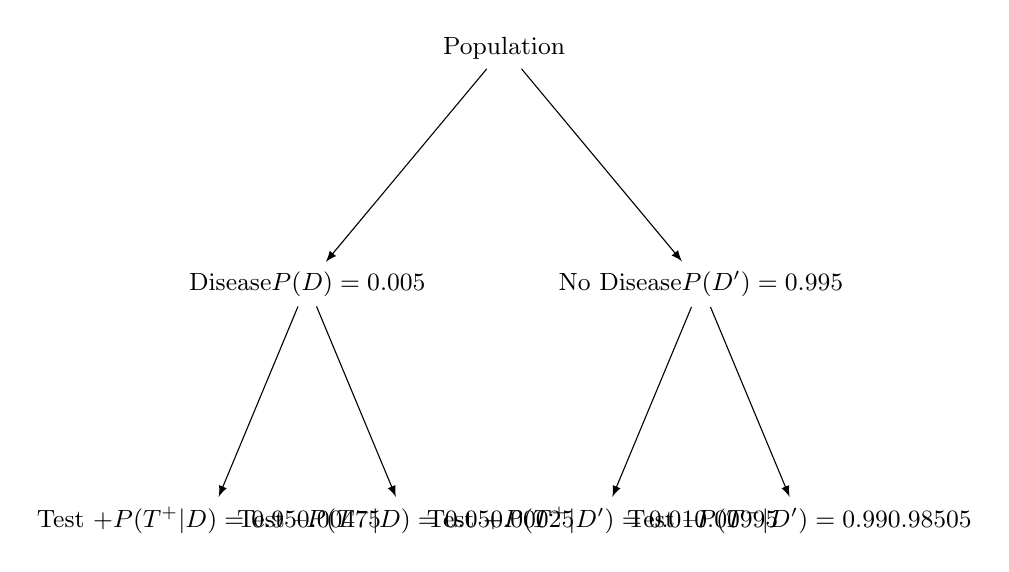
\begin{tikzpicture}[
    level 1/.style={sibling distance=5cm, level distance=3cm},
    level 2/.style={sibling distance=2.5cm, level distance=3cm},
    edge from parent/.style={draw, -latex},
    every node/.style={text centered, font=\small}
]

\node {Population}
    child {node {Disease\\$P(D) = 0.005$}
        child {node {Test +\\$P(T^+|D) = 0.95$\\$0.00475$}}
        child {node {Test --\\$P(T^-|D) = 0.05$\\$0.00025$}}
    }
    child {node {No Disease\\$P(D') = 0.995$}
        child {node {Test +\\$P(T^+|D') = 0.01$\\$0.00995$}}
        child {node {Test --\\$P(T^-|D') = 0.99$\\$0.98505$}}
    };
    
\end{tikzpicture}
\end{center}

\vspace{0.3cm}
The path ``Disease $\to$ Test +'' has probability $0.00475$.

The total probability of testing positive is $0.00475 + 0.00995 = 0.0147$.

Therefore: $P(D|T^+) = \frac{0.00475}{0.0147} = 0.323$.

\end{answer}

\newpage
\section{Additional Questions}

\subsection*{Venn Diagrams}

\begin{question}
Draw Venn diagrams for:
\begin{itemize}
    \item Red and Even numbers on a roulette wheel
    \item Red and Black numbers on a roulette wheel
\end{itemize}
\end{question}

\begin{answer}

\textbf{(a) Red and Even:}

These events overlap (8 numbers are both red and even).

\begin{center}
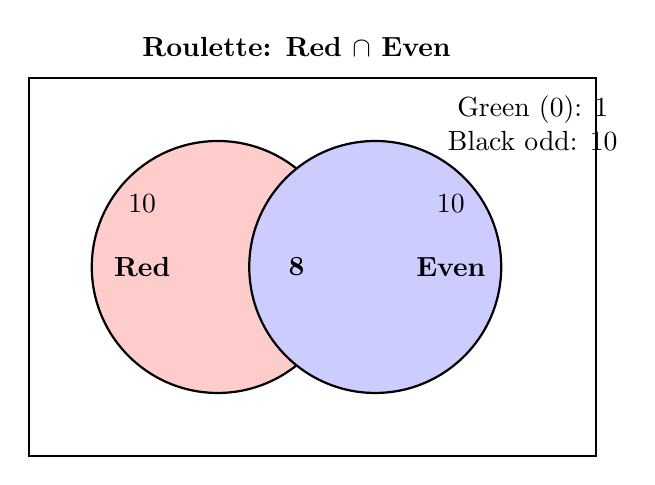
\begin{tikzpicture}[scale=0.8]
    % Draw two intersecting circles
    \draw[thick, fill=red!20] (0,0) circle (2cm);
    \draw[thick, fill=blue!20] (2.5,0) circle (2cm);
    
    % Labels
    \node at (-1.2,0) {\textbf{Red}};
    \node at (3.7,0) {\textbf{Even}};
    \node at (1.25,0) {\textbf{8}};
    \node at (-1.2,1) {10};
    \node at (3.7,1) {10};
    
    % Rectangle for sample space
    \draw[thick] (-3,-3) rectangle (6,3);
    \node at (5,2.5) {Green (0): 1};
    \node at (5,2) {Black odd: 10};
    
    % Title
    \node at (1.25,3.5) {\textbf{Roulette: Red $\cap$ Even}};
\end{tikzpicture}
\end{center}

\begin{itemize}
    \item Red only (odd reds): 10 numbers
    \item Even only (black evens): 10 numbers
    \item Both red and even: 8 numbers
    \item Neither (black odd + green): 9 numbers
\end{itemize}

\vspace{1cm}

\textbf{(b) Red and Black:}

These events are mutually exclusive (no overlap).

\begin{center}
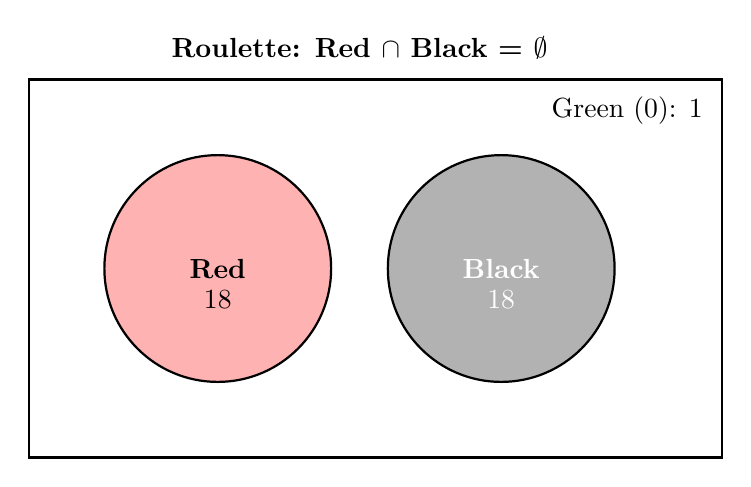
\begin{tikzpicture}[scale=0.8]
    % Draw two non-intersecting circles
    \draw[thick, fill=red!30] (0,0) circle (1.8cm);
    \draw[thick, fill=black!30] (4.5,0) circle (1.8cm);
    
    % Labels
    \node at (0,0) {\textbf{Red}};
    \node at (0,-0.5) {18};
    \node[white] at (4.5,0) {\textbf{Black}};
    \node[white] at (4.5,-0.5) {18};
    
    % Rectangle for sample space
    \draw[thick] (-3,-3) rectangle (8,3);
    \node at (6.5,2.5) {Green (0): 1};
    
    % Title
    \node at (2.25,3.5) {\textbf{Roulette: Red $\cap$ Black = $\emptyset$}};
\end{tikzpicture}
\end{center}

Red and Black are \textbf{mutually exclusive} — they cannot occur simultaneously. Therefore:
\[
P(\text{Red} \cap \text{Black}) = 0
\]
\end{answer}

\subsection*{Union Rule — Do You See Why?}

\begin{question}
For the calculation $P(\text{Red OR Even}) = \frac{18}{37} + \frac{18}{37} - \frac{8}{37} = \frac{28}{37}$, explain why we subtract the 8.
\end{question}

\begin{answer}
\textbf{The Union Rule:}
\[
P(A \cup B) = P(A) + P(B) - P(A \cap B)
\]

\textbf{Why the subtraction?}

When we count all red numbers (18) and all even numbers (18), we've counted the numbers that are \textbf{both red and even twice}:
\begin{itemize}
    \item Once in the ``red'' count
    \item Once in the ``even'' count
\end{itemize}

The 8 red-even numbers are: 12, 14, 16, 18, 30, 32, 34, 36.

To correct for this double-counting, we subtract them once:
\[
18 + 18 - 8 = 28
\]

\textbf{Visual intuition from Venn diagram:}

If you look at the Venn diagram, the overlapping region (intersection) gets counted when you count the left circle \textit{and} when you count the right circle. So after adding both circles, you've counted the overlap twice. Subtracting it once gives you the correct total.

\textbf{General principle:}
\begin{align*}
\text{Total} &= \text{(Only A)} + \text{(Only B)} + \text{(Both A and B)}\\
&= \underbrace{[\text{Only A} + \text{Both}]}_{\text{All of A}} + \underbrace{[\text{Only B} + \text{Both}]}_{\text{All of B}} - \text{Both}\\
&= P(A) + P(B) - P(A \cap B)
\end{align*}
\end{answer}

\subsection*{Conditional Probability}

\begin{question}
For a single spin of a European roulette wheel:
\begin{itemize}
    \item[(a)] What is $P(\text{Black}|\text{Odd})$ — the probability of black given the result is odd?
    \item[(b)] What is $P(\text{Red}|\text{Green})$ — the probability of red given the result is green?
\end{itemize}
\end{question}

\begin{answer}
\textbf{(a) $P(\text{Black}|\text{Odd})$}

By definition of conditional probability:
\[
P(\text{Black}|\text{Odd}) = \frac{P(\text{Black} \cap \text{Odd})}{P(\text{Odd})}
\]

There are 18 odd numbers total. Of these, 10 are black and 8 are red (the green 0 is not odd).

Wait, let me recalculate: there are 18 odd numbers from 1--36 (all odd). Of the 18 black numbers, how many are odd?

Black numbers: 2, 4, 6, 8, 10, 11, 13, 15, 17, 20, 22, 24, 26, 28, 29, 31, 33, 35.

Actually, in European roulette, the specific red/black assignments are:
\begin{itemize}
    \item Among 1--36: 18 are red, 18 are black
    \item Among 1--36: 18 are odd, 18 are even
    \item These are not perfectly distributed
\end{itemize}

Let's use the standard European roulette layout:
\begin{itemize}
    \item Red: 1, 3, 5, 7, 9, 12, 14, 16, 18, 19, 21, 23, 25, 27, 30, 32, 34, 36
    \item Black: 2, 4, 6, 8, 10, 11, 13, 15, 17, 20, 22, 24, 26, 28, 29, 31, 33, 35
\end{itemize}

Odd numbers (1--36): 1, 3, 5, 7, 9, 11, 13, 15, 17, 19, 21, 23, 25, 27, 29, 31, 33, 35 (18 total)

Of these odd numbers:
\begin{itemize}
    \item Red odd: 1, 3, 5, 7, 9, 19, 21, 23, 25, 27 (10 numbers)
    \item Black odd: 11, 13, 15, 17, 29, 31, 33, 35 (8 numbers)
\end{itemize}

Therefore:
\begin{align}
P(\text{Black}|\text{Odd}) &= \frac{P(\text{Black} \cap \text{Odd})}{P(\text{Odd})}\\
&= \frac{8/37}{18/37}\\
&= \frac{8}{18}\\
&= \frac{4}{9}\\
&\approx 0.444
\end{align}

\textbf{Interpretation:} Given that the ball lands on an odd number, there's a $\frac{4}{9}$ chance it's black.

\vspace{0.5cm}

\textbf{(b) $P(\text{Red}|\text{Green})$}

\[
P(\text{Red}|\text{Green}) = \frac{P(\text{Red} \cap \text{Green})}{P(\text{Green})}
\]

A number cannot be both red and green, so:
\[
P(\text{Red} \cap \text{Green}) = 0
\]

Therefore:
\[
P(\text{Red}|\text{Green}) = \frac{0}{1/37} = 0
\]

\textbf{Interpretation:} If we know the ball landed on green (the 0), then the probability it's red is 0. This makes intuitive sense: knowing it's green tells us with certainty it's not red.
\end{answer}

\subsection*{Independence}

\begin{question}
You spin a European roulette wheel twice. Let:
\begin{itemize}
    \item $A$ = ``First spin is red''
    \item $B$ = ``Second spin is even''
\end{itemize}

Are $A$ and $B$ independent? Verify using the definition of independence.
\end{question}

\begin{answer}
\textbf{Definition of Independence:}

Two events $A$ and $B$ are independent if and only if:
\[
P(A \cap B) = P(A) \times P(B)
\]

Equivalently: $P(A|B) = P(A)$ (knowing $B$ doesn't change the probability of $A$).

\vspace{0.3cm}
\textbf{Analysis:}

The two spins are separate physical events. The roulette wheel has no memory — the outcome of the first spin cannot affect the outcome of the second spin.

\begin{align*}
P(A) &= P(\text{first spin is red}) = \frac{18}{37}\\
P(B) &= P(\text{second spin is even}) = \frac{18}{37}\\
P(A \cap B) &= P(\text{first red AND second even})\\
&= P(\text{first red}) \times P(\text{second even})\\
&= \frac{18}{37} \times \frac{18}{37}\\
&= \frac{324}{1369}
\end{align*}

Since $P(A \cap B) = P(A) \times P(B)$, the events are \textbf{independent}.

\vspace{0.3cm}
\textbf{Check using conditional probability:}
\[
P(A|B) = \frac{P(A \cap B)}{P(B)} = \frac{324/1369}{18/37} = \frac{324}{1369} \times \frac{37}{18} = \frac{18}{37} = P(A)
\]

$\checkmark$ Confirmed: $P(A|B) = P(A)$, so $A$ and $B$ are independent.

\vspace{0.3cm}
\textbf{Intuition:}

The second spin doesn't ``know'' what happened on the first spin. The wheel doesn't have memory. Physical independence implies statistical independence.

\vspace{0.3cm}
\textbf{Contrast with non-independent events:}

If instead we had ``first spin is red'' and ``first spin is even'', these would \textit{not} be independent because they both refer to the \textit{same} spin. Knowing the outcome is even tells us something about whether it's red (since 8 out of 18 reds are even).
\end{answer}

\subsection*{Exhaustive Events}

\begin{question}
Consider a single spin of a European roulette wheel. Let:
\begin{itemize}
    \item $B$ = Even
    \item $C$ = Green (0)
    \item $D$ = Odd
\end{itemize}

Are these events exhaustive? That is, is $B \cup C \cup D = S$ (the entire sample space)?
\end{question}

\begin{answer}
\textbf{Definition:} Events are \textbf{exhaustive} if their union covers the entire sample space — i.e., at least one of them must occur.

\vspace{0.3cm}
\textbf{Analysis:}

\begin{align*}
B &= \text{Even} = \{2, 4, 6, 8, 10, 12, 14, 16, 18, 20, 22, 24, 26, 28, 30, 32, 34, 36\}\\
C &= \text{Green} = \{0\}\\
D &= \text{Odd} = \{1, 3, 5, 7, 9, 11, 13, 15, 17, 19, 21, 23, 25, 27, 29, 31, 33, 35\}
\end{align*}

Union:
\[
B \cup C \cup D = \{0, 1, 2, 3, \ldots, 36\} = S
\]

$\checkmark$ \textbf{Yes, these events are exhaustive.}

Every possible outcome is included:
\begin{itemize}
    \item If the ball lands on 0, event $C$ occurs
    \item If the ball lands on an even number (2, 4, ..., 36), event $B$ occurs
    \item If the ball lands on an odd number (1, 3, ..., 35), event $D$ occurs
\end{itemize}

\vspace{0.3cm}
\textbf{Check probabilities:}
\begin{align}
P(B \cup C \cup D) &= P(B) + P(C) + P(D) \quad \text{(mutually exclusive)}\\
&= \frac{18}{37} + \frac{1}{37} + \frac{18}{37}\\
&= \frac{37}{37}\\
&= 1
\end{align}

$\checkmark$ The total probability is 1, confirming the events are exhaustive.

\vspace{0.3cm}
\textbf{Note:} These events are also \textbf{mutually exclusive} (no overlap), so they form a \textbf{partition} of the sample space.
\end{answer}

\newpage
\section{Summary and Key Takeaways}

\subsection*{Fundamental Concepts}

\begin{enumerate}
    \item \textbf{Conditional Probability}
    
    $P(A|B) = \frac{P(A \cap B)}{P(B)}$ — the probability of $A$ given that $B$ has occurred.
    
    \item \textbf{Independence}
    
    Events $A$ and $B$ are independent if $P(A \cap B) = P(A) \times P(B)$, or equivalently, $P(A|B) = P(A)$.
    
    \item \textbf{Union Rule}
    
    $P(A \cup B) = P(A) + P(B) - P(A \cap B)$ — accounts for double-counting the overlap.
    
    \item \textbf{Law of Total Probability}
    
    If $B_1, B_2, \ldots, B_n$ partition the sample space:
    \[
    P(A) = \sum_{i=1}^{n} P(A|B_i) P(B_i)
    \]
    
    \item \textbf{Bayes' Theorem}
    
    \[
    P(A|B) = \frac{P(B|A) P(A)}{P(B)}
    \]
    
    Used to ``reverse'' conditional probabilities — find $P(\text{cause}|\text{effect})$ from $P(\text{effect}|\text{cause})$.
    
    \item \textbf{Mutually Exclusive Events}
    
    Events that cannot occur together: $P(A \cap B) = 0$. For such events: $P(A \cup B) = P(A) + P(B)$.
    
    \item \textbf{Exhaustive Events}
    
    Events whose union covers the entire sample space: $P(A_1 \cup A_2 \cup \cdots \cup A_n) = 1$.
\end{enumerate}

\subsection*{Common Pitfalls (Real-World Cases)}

\begin{enumerate}
    \item \textbf{Assuming Independence Without Justification}
    
    \textit{Sally Clark case:} Two SIDS deaths in the same family are \textbf{not} independent due to shared genetics and environment.
    
    \textit{Lesson:} Always question whether events are truly independent. Correlation in underlying factors creates dependence.
    
    \item \textbf{Post-hoc Analysis \& Selection Bias}
    
    \textit{Lucia de Berk case:} Calculating the probability of a specific pattern \textit{after} observing it is misleading.
    
    \textit{Lesson:} Patterns found by searching through data need correction for multiple testing. ``How likely is this specific pattern?'' is different from ``How likely is it that \textit{some} unusual pattern exists?''
    
    \item \textbf{Prosecutor's Fallacy}
    
    Confusing $P(\text{evidence}|\text{innocence})$ with $P(\text{innocence}|\text{evidence})$.
    
    \textit{Example:} ``The probability of this evidence if she's innocent is 1 in 73 million'' does \textbf{not} mean ``The probability she's innocent is 1 in 73 million.''
    
    \textit{Lesson:} Use Bayes' theorem. You need the \textbf{prior probability} and must account for $P(\text{evidence}|\text{guilt})$ as well.
    
    \item \textbf{Ignoring Base Rates}
    
    \textit{Blood test example:} A 95\% accurate test for a rare disease (0.5\% prevalence) still gives mostly false positives.
    
    \textit{Lesson:} When an event is rare, even a highly accurate test will produce many false positives because there are so many more ``negative'' cases to begin with.
\end{enumerate}

\subsection*{Problem-Solving Strategy}

\begin{enumerate}
    \item \textbf{Define the sample space} — What are all possible outcomes?
    
    \item \textbf{Identify the events of interest} — What exactly are we calculating?
    
    \item \textbf{Check for independence} — Can events influence each other?
    
    \item \textbf{Use appropriate formulas}:
    \begin{itemize}
        \item Union: $P(A \cup B) = P(A) + P(B) - P(A \cap B)$
        \item Independent intersection: $P(A \cap B) = P(A) \times P(B)$
        \item Dependent intersection: $P(A \cap B) = P(A) \times P(B|A)$
        \item Conditional: $P(A|B) = \frac{P(A \cap B)}{P(B)}$
        \item Bayes: $P(A|B) = \frac{P(B|A) P(A)}{P(B)}$
    \end{itemize}
    
    \item \textbf{Draw diagrams} — Venn diagrams, tree diagrams, and tables make structure visible
    
    \item \textbf{Check intuition} — Does the answer make sense? Probabilities must be between 0 and 1. Does the result match your intuition? If not, understand why.
\end{enumerate}

\vspace{0.5cm}

\begin{center}
\textit{``In God we trust. All others must bring data.''} — W. Edwards Deming

\vspace{0.3cm}

\textit{``The purpose of computing is insight, not numbers.''} — Richard Hamming
\end{center}

\end{document}
